\documentclass[11pt,a4paper]{article}
\usepackage[T1]{fontenc}
\usepackage{lmodern}
\usepackage{a4wide}
\usepackage[dvips]{graphicx}
\usepackage{float}

\usepackage[
pdfauthor={ ACE Projekt Team },
pdftitle={ Evaluation Algorithms },
pdfcreator={pdftex},
]{hyperref}

\usepackage{sectsty}
\allsectionsfont{\sffamily}

\usepackage{fancyheadings} 
\pagestyle{fancy} 
\lhead{\textsf{\textbf{ACE} \\ \small{a collaborative editor}}}
\chead{}
\rhead{
\parbox[c]{3cm}{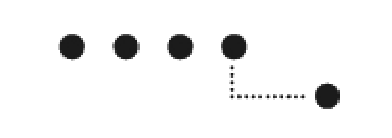
\includegraphics[height=0.875cm,width=3cm]{../../images/logo_BFH.eps}}
\parbox[c]{2.2cm}
{\tiny{\textsf{Berner Fachhochschule \\
Hochschule f�r \\
Technik und Informatik}}}}
\lfoot{}
\cfoot{\textsf{\thepage}}
\rfoot{}
\setlength{\headrulewidth}{0.6pt}
\setlength{\footrulewidth}{0.6pt}
\setlength{\topmargin}{-50pt}
\addtolength{\headheight}{50pt}

\usepackage{colortbl}

\newcommand{\headercol}[2]{\multicolumn{1}{|>{\bfseries\columncolor[gray]{0.82}}p{#1}|}{\textsf{#2}}}
\newcommand{\ace}[0]{\emph{ACE }}



\begin{document}
\setlength{\parindent}{0pt}

\newtheorem{defn}{Definition}
\newtheorem{spec}{Specification}

\bibliographystyle{plain}

\begin{titlepage}
\thispagestyle{empty}
  
\includegraphics[height=1.5in]{../images/pix.eps}

  \begin{center}

    {\fontsize{40}{45} \textbf{\textsf{ACE}}} \\
    \textsf{a collaborative editor} \\
        
    \vspace{36pt}
        
    {\huge{\textbf{\textsf{}}}} \\

    \vspace{36pt}

	\textsf{Berne University of Applied Sciences} \\
    \textsf{School of Engineering and Information Technology} \\
    
  \end{center}

  \vfill
  
  \begin{tabular}{ll}
   \hline

   \\

   \multicolumn{1}{>{\bfseries}p{1.5in}}{\textsf{Date:}} &
   \multicolumn{1}{>{}p{4.3in}}{\textsf{08.11.2005}}          \\
   
   \\
   
   \multicolumn{1}{>{\bfseries}p{1.5in}}{\textsf{Version:}}     &   
   \multicolumn{1}{>{}p{4.3in}}{\textsf{0.1}}                 \\

   \\
   
   \multicolumn{1}{>{\bfseries}p{1.5in}}{\textsf{Projectteam:}}                 &
   \multicolumn{1}{>{}p{4.3in}}{\textsf{Mark Bigler (biglm2@hta-bi.bfh.ch)}}  \\
   \multicolumn{1}{>{\bfseries}p{1.5in}}{}                                      &
   \multicolumn{1}{>{}p{4.3in}}{\textsf{Simon Raess (rasss@hta-bi.bfh.ch)}}    \\
   \multicolumn{1}{>{\bfseries}p{1.5in}}{}                                      &
   \multicolumn{1}{>{}p{4.3in}}{\textsf{Lukas Zbinden (zbinl@hta-bi.bfh.ch)}} \\   
   
   \\
   
   \multicolumn{1}{>{\bfseries}p{1.5in}}{\textsf{Receivers:}}                       &
   \multicolumn{1}{>{}p{4.3in}}{\textsf{Jean-Paul Dubois (doj@hta-bi.bfh.ch)}}       \\
   \multicolumn{1}{>{\bfseries}p{1.5in}}{}                                          &
   \multicolumn{1}{>{}p{4.3in}}{\textsf{Claude Fuhrer (frc@hta-bi.bfh.ch)}}       \\

   \\
   
   \multicolumn{1}{>{\bfseries}p{1.5in}}{\textsf{Location:}}               &   
   \multicolumn{1}{>{}p{4.3in}}{\textsf{Subversion Repository}} \\

   \\  
   
   \hline
  \end{tabular}

\end{titlepage}

\newpage

\tableofcontents
\newpage
\listoftables
\listoffigures
\newpage


\section*{Versionskontrolle}

\begin{table}[!h]
 \begin{tabular}{|l|l|l|l|}
  \hline
  \headercol{0.6in}{Version}         & 
  \headercol{0.8in}{Datum}           &
  \headercol{1.2in}{Verantwortlich}  & 
  \headercol{2.8in}{Bemerkungen}     \\
  \hline
  0.1         & 15.03.2005  & rasss           &  Erste Version \\
  \hline
  0.2         & 22.03.2005  & rasss zbinl     &  �berarbeitung \\
  \hline
  0.3         & 30.03.2005  & zbinl           &  Projektspezifisches Vorgehensmodell \\
  \hline
  0.4         & 30.03.2005  & rasss zbinl     &  �berarbeitung Punkte 2, 3 und 4 \\
  \hline
  0.5         & 05.04.2005  & zbinl           &  �berarbeitung Appendix A.1 \\
  \hline
  0.6         & 06.04.2005  & zbinl           &  Anpassungen Punkte 2, 3 und 4 \\
  \hline
  0.7         & 06.04.2005  & Projektteam     &  Review \\
  \hline
  0.8         & 13.04.2005  & Projektteam     &  Letzte Anpassungen \\
  \hline
  1.0         & 13.04.2005  & Projektteam     &  Freigabe \\
  \hline
 \end{tabular}
 \caption{Versionskontrolle}
 \label{Versionskontrolle}
\end{table}

\begin{table}[!h]
 \begin{tabular}{|l|l|l|l|l|}
  \hline
  \headercol{0.9in}{}            & 
  \headercol{0.9in}{Stelle}      & 
  \headercol{0.8in}{Datum}       & 
  \headercol{0.6in}{Visum}       & 
  \headercol{2.0in}{Bemerkungen} \\
  \hline
  \textbf{Freigegeben}   & Projektteam &       &       &             \\
  \hline
  \textbf{Genehmigt}     &             &       &       &             \\
  \hline
 \end{tabular}
 \caption{Pr�fung/Genehmigung}
 \label{Pr�fung/Genehmigung}
\end{table}

\newpage


\section{Introduction}
Real-time cooperative editing systems allow multiple users to view and edit the same document at the same time from multiple sites connected by communication networks. Consistency maintenance is one of the most significant challenges in designing and implementing real-time cooperative editing systems. 


\subsection{Requirements}
The following requirements have been identified for such systems.

\paragraph{Real-time:} The response to local user actions must be quick, ideally as quick as a single-user editor, and the latency for reflecting remote user actions is low (determined by external communication latency only). 

\paragraph{Distributed:} Cooperating users may reside on different machines connected by communication networks with nondeterministic latency.

\paragraph{Unconstrained:} Multiple users are allowed to concurrently and independently edit any part of the document at any time, in order to facilitate free and natural information flow among multiple users.


\subsection{Preliminaries}
In this section, some basic concepts and terminologies are introduced. Following Lamport\cite{lamport78}, we define a causal (partial) ordering relation on operations in terms of their generation and execution sequences as follows.

\begin{defn}
Causal ordering relation $\rightarrow$
\end{defn}

Given two operations $O_{a}$ and $O_{b}$ generated at sites $i$ and $j$, then $O_{a}\rightarrow O_{b}$, iff:
\begin{enumerate}
 \item $i=j$ and the generation of $O_{a}$ happened before the generation of 
       $O_{b}$
 \item or $i \neq $j and the execution of $O_{a}$ at site $j$ happened before 
       the generation of $O_{b}$
 \item or there exists an operation $O_{x}$ such that $O_{a}\rightarrow O_{x}$
       and $O_{x}\rightarrow O_{b}$
\end{enumerate}

Note that the causal ordering relation is a \emph{partial ordering}.

\begin{defn}
Dependent and independent operations
\end{defn}

Given any two operations $O_{a}$ and $O_{b}$:
\begin{enumerate}
 \item $O_{b}$ is \emph{dependent} on $O_{a}$ iff $O_{a} \rightarrow O_{b}$
 \item $O_{a}$ and $O_{b}$ are \emph{independent} (or \emph{concurrent}), 
       expressed as $O_{a} \Arrowvert O_{b}$ iff neither 
       $O_{a}\rightarrow O_{b}$ nor $O_{b}\rightarrow O_{a}$
\end{enumerate}

Intuitively we can say that two operations are dependant if there exists a path from the generation of one message to the generation of another message. So for example in figure \ref{fig:example1} operation $O_{1}$ and $O_{3}$ are dependent, that is $O_{1}\rightarrow O_{3}$. Operation $O_{1}$ and $O_{2}$ are \emph{independent}. 


\subsection{A shared document model}
Consider $n$ sites, where each site has a copy of the shared document. The shared document model we take is a \emph{text document} modeled a by sequence of characters, indexed from 0 up to the number of characters in the document. It is assumed that the document state (the text) can only be modified by executing the following two primitive editing operations: (i) $Insert(p,c)$ which inserts the character $c$ at position $p$; (ii) $Delete(p)$ which deletes the character at position $p$.

It is important to note that the above text document model is only an abstract view of many document models based on a linear structure. For instance the character parameter may be regarded as a string of charcters, a line, a block of lines, an ordered XML node, etc.


\subsection{Three inconsistency problems}
\label{constraints}

To illustrate the challenges researchers are facing, consider a scenario in a cooperative editing system with three cooperating sites, as shown in figure \ref{fig:example1}. Suppose that an operation is executed on the local replica of the shared document immediately after its generation, then broadcast to remote sites and executed there in its \emph{original form} upon its arrival.
Three different inconsistency problems have been identified by {Sun et. al}\cite{sun98a}.

\begin{figure}
 \centering
 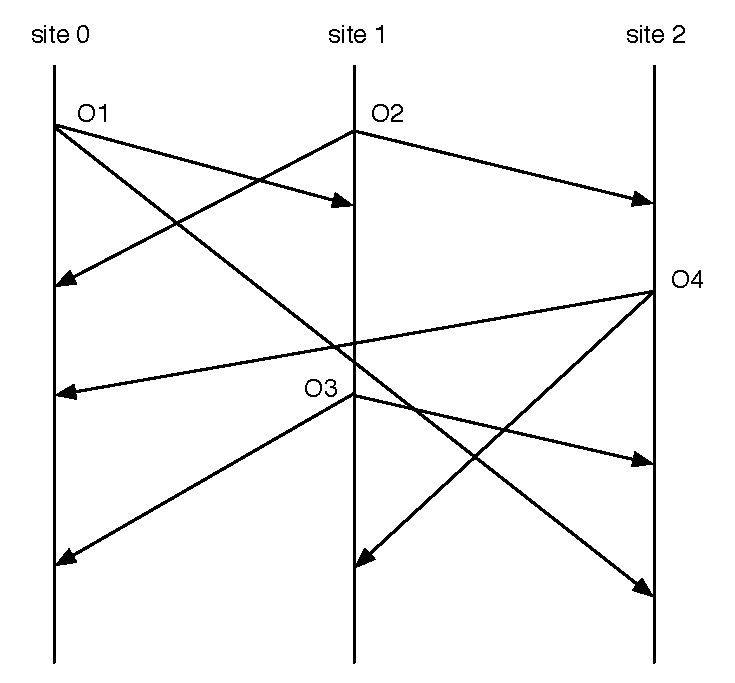
\includegraphics[width=2.5in,height=2.88in]{../../images/example1.eps}
 \caption{A scenarion of a real-time cooperative editing session}
 \label{fig:example1}
\end{figure}

\paragraph{Divergence:}
Operations may arrive and be executed at different sites in different orders, resulting in different final results. As shown in figure \ref{fig:example1}, the four operations in this scenario are executed in the following orders: $O_{1}$, $O_{2}$, $O_{4}$ and $O_{3}$ at site 0; $O_{2}$, $O_{1}$, $O_{3}$ and $O_{4}$ at site 1; and $O_{2}$, $O_{4}$, $O_{3}$ and $O_{1}$ at site 2. Unless operations are commutative, which is generally not the case, final editing results will diverge. The divergence problem can be solved by any serialization protocol, which ensures the final result is the same as if all operations were executed in the same total order at all sites.

\paragraph{Causality violation:}
Due to the nondeterministic communication latency, operations may arrive and be executed out of their natural cause-effect order. As shown in figure \ref{fig:example1}, operation $O_{3}$ is generated after the arrival of $O_{1}$ at site 1, the editing effect of $O_{1}$ on the shared document has been seen by the user 1 at the time $O_{3}$ is generated. Therefore, $O_{3}$ may be \emph{dependent} on $O_{1}$. However, since $O_{3}$ arrives and is executed before $O_{1}$ at site 2, confusion may occure to the system as well as to the user at site 2. For example, if $O_{1}$ is to insert a string into a shared document, and $O_{3}$ is to delete some characters in the string inserted by $O_{1}$, then the execution of $O_{3}$ before $O_{1}$ at site 2 will result in $O_{3}$ referring to a nonexistent context. 

\paragraph{Intention violation:}
Due to concurrent generation of operations, the \emph{actual effect} of an operation at the time of its execution may be different from the \emph{intended effect} of this operation at the time of its generation. As shown in figure \ref{fig:example1}, operation $O_{1}$ is generated at site 0 without any knowledge of $O_{2}$ generated at site 1, so $O_{1}$ is \emph{independent} of $O_{2}$, and vice versa. At site 0, $O_{2}$ is executed on a document state which has been changed by the preceding execution of $O_{1}$. Therefore, the subsequent execution of $O_{2}$ may refer to an incorrect position in the new document state, resulting in an editing effect which is different from the \emph{intention} of $O_{2}$. 

For example, assume the shared document initially contains the following sequence of characters: '"ABCDE'". Suppose $O_{1}=Insert['"12'",1]$, which intends to insert string '"12'" at position 1, i.e. between '"A'" and '"BCDE'"; and $O_{2}=Delete[2,2]$, which intends to delete the two characters starting from position 2, i.e. '"CD'". After the execution of these two operations, the \emph{intention-preserved} result (at all sites) should be: '"A12BE'". However, the actual result at site 0, obtained by executing $O_{1}$ followed by executing $O_{2}$, would be: '"A1CDE'", which apparently violates the intention of $O_{1}$ since the character '"2'", which was intented to be inserted, is missing in the final text, and violates the intention of $O_{2}$ since characters '"CD'", which were intended to be deleted, are still present in the final text.

Even if a serialization-based protocol was used to ensure that all sites execute $O_{1}$ and $O_{2}$ in the same order to get an identical result '"A1CDE'", but this identical result is still inconsistent with the intentions of both $O_{1}$ and $O_{2}$.

\paragraph{} 
The three inconsistency problems are independent in the sense that the occurence of one or two of them does not always result in the others. Particularly, intention violation is an incosistency problem of a different nature from the divergence problem. The essential difference between divergence and intention violation is that the former can always be resolved by a serialization protocol, but the latter cannot be fixed by any serialization protocol if operations were always executed in their originial forms.


\subsection{A consistency model}
A cooperative editing system is said to be consistent if it always maintains the following properties:
\paragraph{Convergence:} when the same set of operations have been executed at all sites, all copies of the shared document are identical.
\paragraph{Causality-preservation:} for any pair of operations $O_a$ and $O_b$, if $O_a \rightarrow O_b$, then $O_a$ is executed before $O_b$ at all sites.
\paragraph{Intention-preservation:} for any operation $O$, the effects of executing $O$ at all sites are the same as the intention of $O$, and the effect of executing $O$ does not change the effects of indepentent operations.

{\setlength{\parskip}{18pt}
In essence, the \emph{convergence} property ensures the consistency of the final results \emph{at the end} of a cooperative editing session; the \emph{causality-preservation} property ensures the consistency of the execution orders of dependent operations \emph{during} a cooperative editing session; and the \emph{intention-preservation} property ensures that executing an opertion at remote sites achieves the same effect as executing this operation at the local site at the time of its generation, and the execution effects of independent operations do not interfere with each other.
}

The consistency model imposes an execution order constraint on dependent operations only. The execution order of independent operations is left open as long as the convergence and intention-preservation properties are maintained. The consistency model effectively specifies, what assurance a cooperative editing system gives to its users and, what properties the underlying consistency maintenance mechanism must support.



\subsection{Operational Transformation}
{Ellis and Gibbs}~\cite{ellis} proposed a new kind of algorithm for consistency control, called \emph{Operational Transformation} (OT).  This kind of algorithm transforms operations to include/exclude the effects of other operations. Intuitively, transformation shifts the position parameter of an operation before execution to incorporate the effects of previously executed operations that it was not "aware" of (or that are concurrent) at the time of generation. Operational transformation helps to solve the problem of intention violation.

In general there are two different types of operational transformation, inclusion transformation (IT) and exclusion transformation (ET). All OT algorithms use inclusion transformation, whereas exclusion transformation is not needed by some algorithms.

A transformation function has to be defined for every combination of operations. So for a text editor with the primitive operations \emph{insert} and \emph{delete}, there would be a total of four transformation functions for IT and another four for ET. That is, given a transformation function T, T(\emph{insert, insert}), T(\emph{insert, delete}), T(\emph{delete, insert}) and T(\emph{delete, delete}) must be defined.

\subsubsection{Definitions}
\label{definitions}
Conceptually, an operation $O$ is associated with a \emph{context}, denoted as $CT_{O}$, which is the list of operations that need to be executed to bring the document from its initial state to the state on which $O$ is defined (\emph{definition context}). The significance of context is that the effect of an operation can be correctly interpreted only in its own context. If the current context (called \emph{execution context}) is different from the definition context of an operation, the operation has to be transformed so that it can be executed in the current context.

\begin{defn}
Context equivalent relation $\sqcup$
\end{defn}

Given two operations $O_{1}$ and $O_{2}$, associated with contexts $CT_{O_{1}}$ and $CT_{O_{2}}$ respectively, $O_{1}$ and $O_{2}$ are \emph{context-equivalent} iff $CT_{O_{1}}=CT_{O_{2}}$. Apparently, the context equivalent relation $\sqcup$ is transitive.

\begin{defn}
Context preceding relation $\mapsto$
\end{defn}
Given two operations $O_{1}$ and $O_{2}$ associated with contexts $CT_{O_{1}}$ and $CT_{O_{2}}$ respectively, $O_{1}$ is \emph{context preceding} $O_{2}$ iff $CT_{O_{2}}=CT_{O_{1}} + [O_{1}]$. Note that the contex preceding relation $\mapsto$ is not transitive by definition.

\subsubsection{Inclusion Transformation}
Inclusion Transformation (IT) transforms an operation $O_{1}$ against another operation $O_{2}$ in such a way that the impact of $O_{2}$ is effectively included. 
\begin{spec}
$IT(O_a,O_b):O'_a$
\end{spec}
\begin{enumerate}
 \item Precondition for input parameters: $O_a \sqcup O_b$
 \item Postcondition for output: $O_b \mapsto O'_a$ where $O'_a$'s execution effect in the context of $CT_{O'_a}$ is the same as $O_a$'s execution effect in the context of $CT_{O_a}$.
\end{enumerate}

Most important, it was recognized that the correctness of IT relies on the condition that both $O_{1}$ and $O_{2}$ are defined on the same document state so that their parameters are comparable and can be used to derive a proper adjustment to $O_{2}$, i.e. $O_{1} \sqcup O_{2}$.

\subsubsection{Exclusion Transformation}
Exlusion Transformation (ET) transforms an operation $O_{1}$ against another operation $O_{2}$ in such a way that the impact of $O_{2}$ is effectively excluded from $O_{1}$.
\begin{spec}
$ET(O_a,O_b):O'_a$
\end{spec}
\begin{enumerate}
 \item Precondition for input parameters: $O_b \mapsto O_a$
 \item Postcondition for output: $O_b \sqcup O'_a$ where $O'_a$'s execution effect in the context of $CT_{O'_a}$ is the same as $O_a$'s execution effect in the context of $CT_{O_a}$.
\end{enumerate}

Both transformation functions must meet the \emph{reversibility} requirement as defined next.

\subsubsection{Reversibility}
\begin{defn}
Reversibility Requirement
\end{defn}

Given two operations $O_{1}$ and $O_{2}$.

\begin{enumerate}
 \item if $O_{1} \sqcup O_{2}$ and $O'_{1} = IT(O_{1},O_{2})$, then it must
       be that $O_{1} = ET(O'_{1},O_{2})$
 \item if $O_{2} \mapsto O_{1}$ and $O'_{1} = ET(O_{1},O_{2})$, then it must
       be that $O_{1} = IT(O'_{1},O_{2})$
\end{enumerate}

Achieving reversibility is not a trivial task. This is because IT/ET functions may loose some information, so reversing the effect of a transformation may not be possible.


\subsection{Transformation Properties}
It was shown in \cite{ressel96} that transformation functions must satisfy two conditions, called $TP1$ and $TP2$. These transformation properties are sufficient and necessary for OT algorithms to guarantee convergence along arbitrary transformation paths.

\paragraph{Transformation Property 1:}
The transformation property 1 ensures that the effect of executing $O_{1}$ followed by the transformed request $O_{2}$ is the same as executing request $O_{2}$ followed by the transformed request $O_{1}$. 

\begin{defn}
Transformation Property 1:
$ O_{1} O'_{2} \equiv O_{2} O'_{1} $
\end{defn}

\paragraph{Transformation Property 2:}
Transformation property 1 is a necessary and sufficient condition to ensure that the groupware system with two users is correct. When there are more than two users, the situation is more complex. An operation can be transformed along different, albeit equivalent paths, not necessarily yielding the same result. In the simplest case, an operation can be transformed along the two paths of a simple transformation step. Operation $O_{1}$ may be transformed first with respect to $O_{2}$ and then to $O'_{3}$ yielding $IT(IT(O_{1},O_{2}),O'_{3})$, or it may be transformed first with respect to $O_{3}$ and then to $O'_{2}$ yielding $IT(IT(O_{1},O_{3}),O'_{2})$. Note that different sites might choose different paths for $O_{1}$ to be transformed. So we have to make sure that both paths lead to the same resulting operation:

\begin{defn}
Transformation Property 2: 
$IT(IT(O_{1},O_{2}),O'_{3})$=$IT(IT(O_{1},O_{3}),O'_{2})$
\end{defn}


\subsection{Groupware Architecture Analysis} We consider the architecture of a groupware application from two different point of views. On the one hand, the focus lies on the document replication and on the other, we consider the type of group communication between the participating sites.

\subsubsection{Document replication}

\paragraph{Centralized architecture} In a centralized architecture all data, i.e. the document, resides on a central machine. Client processes at each site are only responsible for passing requests to the central program and for displaying any output sent to them from the central program. The advantage of a centralized scheme is that synchronization is easy. Document state information is consistent since it is located in one place, and events are handled at clients in the same order because they are serialized by the server. Its main drawback is latency, as the message corresponding to any action must pass from the client to the server and back again before response to the action is shown.

\paragraph{Replicated architecture} In a replicated architecture the document is replicated at all participating sites. Client processes at each site (replicas) must coordinate explicitly both local and remote actions, synchronizing all copies of the document. Replicas need only exchange critical state information to keep their copy of the document current. While remote activities may still be delayed, local activities can be processed immediately. Processing bottlenecks are less likely, because each replica is responsible for drawing only the local view. The most significant cost of replication is increased complexity as issues of distributed systems like conflict management, concurrency control, etc. must be handled. 

The \emph{real-time} requirement has led most researchers to adopt a replicated architecture.


\subsubsection{Group Communication}
We consider two types of group communication architectures: unicast and multicast:

\paragraph{Unicast communication} Unicast communication is a two way communication where client processes at each site communicate bidirectionally with a centralized server. The server forwards information from one client to all other clients.

\paragraph{Multicast communication} Mulitcast communication is an $n$ way communication where client processes at each site communicate with all the participating sites directly. It has an enormous growth in terms of the number of communication paths. They grow at the rate of $n(n-1)/2$, where $n$ is the number of clients in the system. As compared to this, systems that use unicast communication have a linear growth. 


\section{History}
{Ellis and Gibbs}~\cite{ellis} were the first to propose an \emph{Operational Transformation} algorithm in 1989. The algorithm is called \emph{dOPT} and is implemented in the \emph{Grove} system. Soon however a flaw was discovered in the original \emph{dOPT} algorithm (by Cormack\cite{cormack95a}). The scenario where \emph{dOPT} failed is called the \emph{dOPT} puzzle. Ressel\cite{ressel96} proposed a new algorithm \emph{adOPTed} in 1996 that solved the original \emph{dOPT} puzzle. {Sun et. al}\cite{sun98a} proposed another algorithm called \emph{GOT} that similarly to \emph{adOPTed} solved the \emph{dOPT} puzzle. {Sun et. al}\cite{sun98b} developed some transformation functions for string-wise operations.

Later research groups\cite{imine03}\cite{imine04} proved the transformation functions of both Ressel\cite{ressel96} and Sun\cite{sun98a} to fail to hold TP2 in certain situations. They proposed new transformation functions they developed using a theorem prover. 

Proving the transformation property 1 (TP1) seems to be rather straightforward. However, proving that a given transformation function holds TP2 appears to be difficult. There are over 100 cases that have to be analyzed (according to {Imine et. al}\cite{imine04}). Imine et. al showed that many proposed transformation functions do not hold TP2. 

Recently, two different ways have been taken to deal with the TP2 problem. One kind of algorithms tries to avoid the need to comply with TP2 altogether (GOT~\cite{sun98a}, SOCT3/4~\cite{suleiman00}, TIBOT\cite{tibot} and NICE~\cite{sun02}). Other research groups~\cite{li04}~\cite{imine04} try to correct the problems in the original transformation functions of GOTO~\cite{sun98b}, adOPTed~\cite{ressel96} and SDT~\cite{sdt}. 


\section{Algorithms}
\label{algos}
In this section we give an overview of the \emph{Operational Transformation} algorithms we could gather. Two important properties on such algorithms are described first.

\paragraph{} The OT algorithm approach consists of two main components:

\begin{enumerate}
 \item The \emph{integration algorithm} which is responsible of receiving, broadcasting and executing operations. It is independent of the type of replica and application.
 \item The \emph{transformation function} is responsible for merging two concurrent operations. It is application dependent. For example, a text editor has different operations than a whiteboard application.
\end{enumerate}

The integration algorithm calls the transformation function when needed. The correctness of the OT approach relies on both the correct integration algorithm as well as on the correct transformation function.

\subsection{dOPT}
\label{algo:dopt}

\emph{dOPT} (Distributed Operational Transformation) is the first operational transformation algorithm developed by {Ellis and Gibbs}\cite{ellis} in 1989. It was soon discovered that in some situations the document replicas did not converge. This situation is known as the \emph{dOPT} puzzle.

The algorithm fails in cases where there is more than one concurrent operation from a user (see figure \ref{fig:doptpuzzle}). Given operation $O_{a}$ from site $a$ and operations $O_{b_{1}}$ and $O_{b_{2}}$ from site $b$, where $O_{a} \parallel O_{b_{1}}$, $O_{a} \parallel O_{b_{2}}$ and $O_{b_{1}} \rightarrow O_{b_{2}}$, \emph{dOPT} incorrectly applies inclusion transformation against $O_{b_{1}}$ and $O_{b_{2}}$ in sequence against $O_{a}$ at site $a$. Note however that $O_{b_{2}}$ is not context-equivalent with $O_{a}$ and therefore $IT(O_{a},O_{b_{2}})$ violates the precondition of inclusion transformation.

\begin{figure}[H]
 \centering
 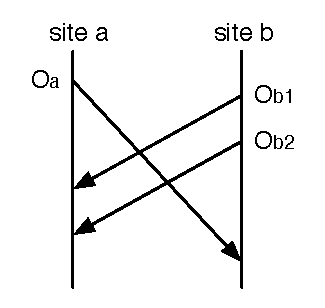
\includegraphics[width=1.94in,height=1.83in]{../../images/dopt_puzzle.eps}
 \caption{dOPT puzzle}
 \label{fig:doptpuzzle}
\end{figure}

Cormack\cite{cormack95a} detected this case and proposed a new algorithm (see \ref{algo:ccu}) that is only suitable for two sites connected by a point-to-point communication channel. He stated that there does not appear to be a simple and efficient correction to \emph{dOPT} that maintains its suitability for broadcast operations.

However Cormack showed in \cite{cormack95b} that using several point-to-point communication channels forming a tree it is possible to derive a consistent solution for an arbitrary number of sites (see also \ref{algo:netedit}).

\subsubsection{Properties}
\begin{itemize}
 \item algorithm is incorrect
 \item uses state vectors to maintain causal ordering
 \item uses linear history buffer (called request log)
 \item architecture: fully replicated
\end{itemize}

\subsection{CCU}
\label{algo:ccu}

CCU (a Calculus for Concurrent Update) derives from the \emph{dOPT} (see \ref{algo:dopt}) algorithm. It was developped by Gordon V.Cormack in 1995 that discovered earlier \cite{cormack95a} that \emph{dOPT} is incorrect. 

The algorithm specifies a concurrent model based on a sequential model augmented with definitions of all possible pairs of elementary operations (updates). The concurrent model is implemented by a set of objects: one for each source of events.

Although there is a description of the algorithm in \cite{cormack95b}, many implementation details are left out. Interestingly no references to this algorithm are found in the other research material. 

\subsubsection{Properties}
\begin{itemize}
 \item correctness never confirmed by other reaserchers
 \item uses state vectors to maintain causal ordering
 \item architecture: semi-replicated (central server)
\end{itemize}

\subsection{Jupiter}
\label{algo:jupiter}

\emph{Jupiter} is a multi-user, multimedia virtual world intended to support long-term remote collaboration. In particular, it supports shared documents, shared tools, and, optionally, live audio/video communication. It is basically a collaborative windowing toolkit. The low-level communication facilities (operational transformation) are described in \cite{jupiter95}.

\emph{Jupiter}'s algorithm is derived from \emph{dOPT}. The centralized architecture and thus the reduction of point-to-point connections allows them to simplify the \emph{dOPT} algorithm. Several point-to-point connections are used to build a tree-structured $n$-site algorithm.

\emph{Jupiter} solves the \emph{dOPT} puzzle. It uses a two dimensional state space instead of a linear history buffer (request log) to save operations. It transforms saved messages against conflicting incoming messages. Unfortunately, simply transforming saved messages does not work for the $n$-way case, since the next message can come from a third site that is in an inconvenient message state. See \emph{adOPTed} \ref{algo:adopted} for a solution to the $n$-way case.


\subsubsection{Details}

The general tool for handling conflicting (concurrent) messages is the transformation function, called \emph{xform} in \cite{jupiter95}.

$$ xform(c,s)={c',s'} $$

It takes a message $c$ from the client and a message $s$ from the server and returns two transformed messages $c'$ and $s'$. The messages $c'$ and $s'$ have the property that if the client applies $c$ followed by $s'$, and the server applies $s$ followed by $c'$, both client and server wind up in the same final state. The \emph{xform} function is basically a combined inclusion transformation (IT) function that returns the result of both $IT(c,s)$ and $IT(s,c)$.

It is helpful to show the two dimensional state space that both client and server pass through as they process messages (see figure \ref{jupiter:statespace1}). Each state is labelled with the number of messages from the client and server that have been processed to that point. For instance if the client is in the state $(2,3)$, it has generated and processed two messages of its own, and has received and processed three from the server. The client and server messages represent different axis in the state space. 

If there is a conflict, the paths will diverge, as shown in figure \ref{jupiter:statespace1}. The client and server moved to the state $(1,1)$ together by first processing a client message, and then a server message. At that point, the client and server processed different messages (concurrently), moving to state $(2,1)$ and $(1,2)$ respecitvely. They each received and processed the other's message using the transformation function to move to state $(2,2)$. Then the server generated another message, sending it to the client and both were in state $(2,3)$.

\begin{figure}[H]
  \centering
  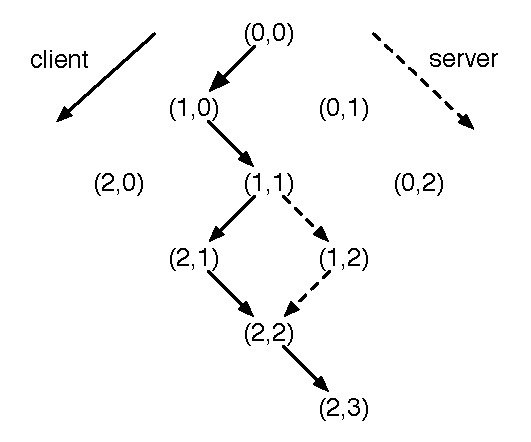
\includegraphics[width=3in,height=2.45in]{../../images/jupiter2.eps}
  \caption{Two dimensional state space example}
  \label{jupiter:statespace1}
\end{figure}

The algorithm labels each message with the state the sender was in just before the message was generated (state vector). The recipient uses these labels to detect conflicts. Two concurrent messages have to be transformed, but they can only be transformed directly when they were generated from the same state of the document. 

If client and server diverge more than one step, the transformation function cannot be applied directly. Consider figure \ref{jupiter:statespace2}. The client has executed $c$ and receives the conflicting message $s1$ from the server. It uses the transformation function to compute $s1$ to get to the state $(1,1)$. The server then generates $s2$ from the state $(0,1)$, indicating that it still has not processed $c$. What should the client do now? It cannot use the transformation function directly because $c$ and $s2$ were not generated from the same document state.

\begin{figure}[H]
 \centering
 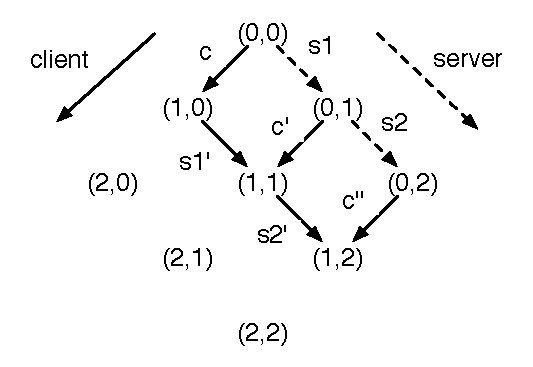
\includegraphics[width=3in,height=2in]{../../images/jupiter.eps}
 \caption{Conflicting messages}
 \label{jupiter:statespace2}
\end{figure}

To solution to this situation is as follows. When the client computes $s1'$ it must also remember $c'$. This represents a hypothetical message that the client could have generated to move from the state $(0,1)$ to $(1,1)$. When $s2$ arrives, the client can use $c'$ to compute $c''$. It executes $s2'$ to get to the state $(1,2)$. If the server has processed the client's message, it will be in the state $(1,2)$ as well. If not, its next message will originate from $(0,3)$, so the client saves $c''$ just in case.

The algorithm guarantees that, no matter how far the client and server diverge in state space, when they do reach the same state, they will have identical states (so convergence is achieved).


\subsubsection{Properties}
\begin{itemize}
 \item seems to be correct
 \item uses state vectors to decide causality relations
 \item architecture: semi-replicated (central server)
 \item uses multiple 2-way synchronization protocols to create a n-way protocol
 \item free of TP2
 \item very simple algorithm
\end{itemize}

\subsection{NetEdit Consistency Algorithm}
\label{algo:netedit}

\emph{NetEdit} is a collaborative text editor (\cite{netedit}) that uses a replicated architecture with processing and data distributed across all clients. It uses an $n$-way synchronization protocol derived from the algorithm of the \emph{Jupiter} (see \ref{algo:jupiter}) collaboration system. The algorithm is called \emph{NetEdit Consistency Algorithm}.

The 2-way synchronization protocol developed for \emph{Jupiter} was the starting point. That algorithm was extended to a multi-way protocol using multiple 2-way connections. In \cite{netedit:thesis}, the multi-way protocol that was already mentioned in \cite{jupiter95} is described in detail.

\subsubsection{Properties}
\begin{itemize}
 \item architecture: semi-replicated (central server)
 \item seems to be correct
 \item uses state vectors to decide causality relations
 \item uses multiple 2-way synchronization protocols to create a n-way protocol
 \item free of TP2
\end{itemize}


\subsection{adOPTed}
\label{algo:adopted}

\emph{adOPTed} was devised by Ressel and Gunzenhaeuser and described in \cite{ressel96}. It is an improved version of the \emph{dOPT} algorithm. A multi-dimensional model of concurrent interaction is the core of this approach. This model allows direct communication with $n$ sites. The algorithm is conceptually similar to \emph{Jupiter} (see \ref{algo:jupiter}), but extends the two way communication in \emph{Jupiter} to a multi way communication. Both use a state space graph to track operations. The state space graph in \emph{adOPTed} is $n$-dimensional wherelse in \emph{Jupiter} it is two dimensional.


\subsubsection{Algorithm}
This algorithm uses a so called \emph{L-Transformation} function. This L-Transformation function is the equivalent of the $xform$ function in \emph{Jupiter} (see \ref{algo:jupiter}) in \emph{adOPTed}. It is defined as:

\label{algo:adopted:tf}
$$ tf(r_1,r_2) = (r'_1,r'_2) $$

An L-transformation function must satisfy TP1 and must be symmetric. Requests and L-transformations can be represented as grid-based diagrams. The axes represent users, grid points represent states with a certain state vector, and arrow represent requests, being either original or the result of some transformation.

Each user process manages the following local data structures: the application state $s$, a counter $k$ for locally generated requests, a site's state vector $v$, its request queue $Q$, a request log $L$ and an n-dimensional interaction model $G$. The \emph{state vector v} holds the number of execution for each user. The $request queue Q$ is used to store generated and incoming requests that have to wait for execution. The \emph{request log L} stores a copy of each original request so that a request can be easily accessed by its key consisting of user id $u$ and serial number $k$. The \emph{interaction model G} is mainly used to store transformed requests that might be needed later. It would be possible to store application states like in the formal definition of the interaction model, but this is not necessary for the algorithm to work.


\subsubsection{Transformation Functions}
In \cite{ressel96} they also propose a set of transformation functions for text editing. There are two operations, insert and delete, so there must be four transformation functions. The transformation functions were proved to be wrong by \cite{imine03}. That is, they do not hold transformation property 2 (TP2). 

Note however that it has been proved by \cite{cormack02} that the control algorithm of \emph{adOPTed} is correct as long as the transformation functions hold TP2. Using the proposed transformation functions from \emph{imine04} results in a correct system that achieves the three properties convergence, causality preservation and intention preservation.


\subsubsection{Properties}
\begin{itemize}
 \item proved to be correct if transformation functions hold TP2
 \item uses state vectors to decide if operations are concurrent
 \item uses only inclusion transformation (IT)
 \item user undo described by \cite{ressel99}
 \item n-dimensional interaction graph
 \item architecture: replicated (no central server needed)
 \item time complexity for integrating a remote operation $O$ is $O(n)$ 
       where $n$ is the number of messages
\end{itemize}


\subsubsection{Known implementations}
Ressel implemented a prototypical group editor named \emph{Joint Emacs}. Another group editor that uses \emph{adOPTed} is \emph{Gclipse}, a collaborative editor plug-in for eclipse.

\subsection{GOT}
\label{algo:got}

\subsection{GOTO}
\label{algo:goto}

\subsection{SOCT2}

\subsection{SOCT3}
\label{algo:soct3}

Verifying that a given set of transformation functions satiesfies transformation property 2 (TP2) is not trivial. There are over a hundred cases to be checked depending on the various parameters. So the inventors of \emph{SOCT3} and \emph{SOCT4} (see \ref{algo:soct4}) decided to go a different way in order that they can abandon TP2 (\cite{suleiman00}).

They propose the implementation of a global serialization order such that the operations can be delivered in this order. The global serialization order is achieved by the use of a sequencer (see \ref{sequencer}). A sequencer is an object which delivers continously growing positive integer values, called timestamps. A timestamp is obtained through a call to a function \emph{Ticket}.

A local operation $O$ is executed immediately to respect the real-time constraint. Next, the call to the function \emph{Ticket} returns a timestamp $N_{O}$ which is assigned to the operation. The quadruplet $<O,S_{O},V_{O},N_{O}>$ is then broadcast where $V_{O}$ is the state vector associated with $O$ and $N_{O}$.

The reception procedure ensures a sequential delivery of all operations with respect to the ascending order of the timestamps. Upon receiving an operation the reception procedure delays its delivery until all operations with lower timestamps have been received and delivered. The state vector is of no use for the reception procudre, but it enables to determine which operations are concurrent to $O$ during the integration step.

\emph{SOCT3} uses both inclusion transformation IT (called forward transposition) and exclusion transformation ET (called backward transposition) in the integration step. For details, see \cite{suleiman00}.


\subsubsection{Properties}
\begin{itemize}
 \item uses state vectors to determine concurrent operations
 \item uses linear history buffer (called history)
 \item architecture: fully replicated
 \item uses a unique global ordering to abandon TP2 (by using a sequencer)
 \item no known user undo algorithm
\end{itemize}

\subsection{SOCT4}

\subsection{TIBOT}
\label{algo:tibot}

The \emph{TIBOT} algorithm presents a novel interaction model that is based on time intervals. It was presented in 2004 by Rui Li, Du Li and Chengzheng Sun in \cite{tibot}. In this summary, firstly some necessary concepts are introduced. Secondly the consistency control algorithm is explained.

\subsubsection{Concepts}
\paragraph{Time intervals based on logical clocks}
Every site in the replicated architecture maintains a linear logical clock. All clocks are initialized to a common value. A time interval is the period between two consecutive clock ticks. Time interval lengths are assumed to be the same. Every operation is timestamped by the current local clock value to indicate which time interval it belongs to. Function $TI(O)$ denotes the time interval of operation $O$. Two operations, $O_{i}$ and $O_{j}$, are in the same time interval iff $TI(O_{i}) = TI(O_{j})$, no matter whether $i = j$ or not. A new time interval at a site is announced by broadcasting a control message that carries the clock value of the new time interval to all remote sites.

\paragraph{Total ordering and operation context}
The total ordering is defined by means of the time interval function.  In addition, \emph{TIBOT} uses a linear history buffer in which the operations are stored in the total order at each site. The notion of operation context is the same as defined in \ref{definitions}. The operations are allowed to be executed in any order as long as their causality is preserved and the following synchronization rules are observed.

\paragraph{Propagation and synchronization rules}
\begin{itemize}
 \item Propagation rule 1: A local operation is propagated only when the current time interval is over and the operation has been transformed with all operations that have been executed in earlier time intervals. That is, a local operation always needs to be transfomred against all operations generated in previous time intervals before it can be propagated. Hence operation propagation is normally delayed.
 \item Propagation rule 2: When a time interval is over, if no operation has been generated locally, a message is propagated to notify other sites that there was no operation generated in the past time interval. 
 \item Synchronization rule 1: Any remote operation received during a time interval can be synchronized only when (1) local time interval is over, if the time interval of this operation is the same as the current local time interval; and (2) all operations totally preceding this operation have been executed.
 \item Synchronization rule 2: When a remote operation is to be executed, all operations that have been executed but out of the total order must be first undone, then perform this operation, and then redo these undone operations in sequence. These operations to be done or redone need to be transformed before they are executed (undo/do/redo scheme). Local operations are always executed immediately once generated.
 \item Synchronization rule 3: Operations with the same timestamp and site id are always synchronized as an entirety (i.e. are processed as entirety in transformations against local operations (concept of group operation).
\end{itemize}
The above rules reduce the complexity of communication and interaction compared with other consistency models for group editors. E.g. exclusion transformation is not necessary in this model.

\subsubsection{The TIBOT control algorithm}
Due to the rules defined above and the properties derived from these rules (see \cite{tibot}), the concurrency problem is simplified in this model. It can be reduced (from the three cases discussed in \cite{sun98b}) to the following two cases. Assume that O is a execution-ready operation. $[O_{1},O_{2},...,O_{n}]$ are a sequence of operations that have been executed locally and stored in the local history buffer (HB). Suppose HB = $[O_{1},O_{2},O_{3}]$.
\begin{itemize}
 \item Case 1: $O_{1} \rightarrow O, O_{2} \rightarrow O, O_{3} \rightarrow O$ \\
 All operations in HB are preceding O. Therefore O' = O, i.e., no transformation is needed.
 \item Case 2: $O_{1} \rightarrow O, O_{2} \parallel O, O_{3} \parallel O$ \\
 Operations preceding O are stored in HB before operations that are independent of O. Then O' is obtained by transforming O against concurrent operations, $O_{2}$ and $O_{3}$, in a sequel.
\end{itemize}

The top-level control algorithm \emph{TIBOT} is based on these two cases and the undo/do/redo scheme. \emph{TIBOT} is called only when a remote group operation is ready for synchronization.


\subsubsection{Properties}
\begin{itemize}
 \item simplified and efficient approach based on time intervals instead of state vectors
 \item uses only inclusive transformation
 \item is free from TP2
 \item time complexity \emph{O(n)}
 \item replicated architecture
 \item implementation of time interval concept not clear
\end{itemize}
\subsection{NICE}
\label{algo:nice}

Haifeng Shen and Chengzhen Sun devised a new operational transformation control algorithm in combination with a notification component in 2002 \cite{sun02}. In this paper they describe a flexible notification framework that can be used to implement a wide range of notification strategies used in collaborative systems.

In the proposed framework, the notification policy that determines when and what to notify is separated from the notification mechanism that determines how to notify. The parameters \emph{frequency} and \emph{granularity} are provided to define various notification policies. 

The frequency parameter determines the \emph{when} aspect of notification, that is, when a notification is propagated/accepted. The granularity parameter determines the \emph{what} aspect of notification, that is, which updates are going to be propagated/accepted. Further there can be a separate policy for input and output direction.

The notification mechanism determines the \emph{how} aspect. Both outgoing and incoming messages are put in distinct buffers (input buffer IB and output buffer OB). An outgoing notification executor (ONE) and an incoming notification executor (INE) are needed to carry out various outgoing and incoming notification policies respectively.

A very important component in the notification mechanism is the notification propagation protocol (NPP), which is needed for propagating updates from the OB at the notifying site to the IB at the notified site.

The notifications are contextually serialized. This is achieved by use of a central notification server, which acts as a centralized serialization point and message relaying agent (all messages pass through this central server). 


\subsubsection{Notification Propagation Protocol}
Before propagating a notification, the notifying site sends a \emph{Token-Request} message to the \emph{Notifier}, waiting for the \emph{Token-Grant} message from the \emph{Notifier}. After being granted the token, the site propagates the notification piggybacked with the \emph{Token-Release} message to the \emph{Notifier}. When the \emph{Notifier} receives the notification and the \emph{Token-Release} message, it forwards the notification to all interested sites. By using the notifier as a message relaying agent, causal relationships among notifications are automatically guaranteed.

This sequential propagation simplifies concurrency control. However it is also inefficient for supporting notification policies for meeting real-time collaboration needs. For propagating one notification that may contain only one operation, three extra messages have to be sent.


\subsubsection{Concurrent Propagation}
So the proposed solution consists of a protocol that allows a site to propagate its notification without first requesting a token, thus effectively eliminating the \emph{Token-Request} message. This operation propagation protocol is called \emph{SCOP} (symmetric contextually-serialized operation propagation). 


\subsubsection{Properties}
The transformation control algorithm is called \emph{SLOT} (symmetric linear operation transformation). Together with the \emph{SCOP} protocol it has the following properties.

\begin{itemize}
 \item architecture: semi-replicated (uses central notification server)
 \item no state vectors needed
 \item no exclusion transformation (ET)
 \item free of transformation property 2 (TP2)
\end{itemize}

The reason why \emph{SLOT} is free of TP2 is that under no circumstance an operation could be transformed against the same pair of operations in different orders. The operation are always ordered uniquely.


\subsection{SDT}
\label{algo:sdt}

The algorithm \emph{SDT} was presented in 2004 by Du Li and Rui Li \cite{sdt}. They detected defects in existing inclusion transformation and exclusion transformation functions. 

\subsubsection{Defects of traditional transformation functions}
The problem is related to inclusion transformation between two insert operations and one delete operation with close position parameters. In some of these cases, the result of inclusion transformation is not deterministic. 

\paragraph{Example: } Given the initial document state ''abc''. The three editing sites 1, 2 and 3 generate $O_{1} = insert(''1'',2)$, $O_{2} = insert(''2'',1)$ and $O_{3} = delete(''b'',1)$ respectively. The three operations are independent. Now consider what happens at site 3. After the deletion of character ''b'' at position 1 the document state becomes ''ac''. The next message arriving is then $O_{2}$ which inserts ''2'' at position 1. The resulting document state is ''a2c''. The next operation $O_{1}$ arrives at site 3 and is transformed against $O_{3}$ and then $O_{2}$. The result of the second transformation is non-deterministic. It could be $insert(''1'',1)$ or $insert(''1'',2)$. However, the original intention of $O_{1}$ is to insert ''1'' after ''b'' and the intention of $O_{2}$ is to insert ''2'' before ''b''. Then ''1'' should appear after ''2'' in the resulting document state (''a21c''). So depending on the chosen priority scheme, the result could be violating the intention of the original operations. Another even more severe problem results from the fact, that the document state of site 3 could diverge from site 1 and 2. A similar problem arises with traditional exclusion transformation functions.

The conventional transformation functions use the site id as priority scheme if two inserts happen at the same position. This was identified as the source of the problems as described above by Du Li and Rui Li. This new algorithm tries to delay the use of site ids.


\subsubsection{Proposed Solution}
In the paper \cite{sdt} they propose a solution to the identified consistency problems. The algorithm works conceptually as follows. For each operation the original intention is recovered by computing its $\beta$ value against a well-known document state (the latest synchronization point). Then in performing inclusion transformation, the $\beta$ values are compared. The approach is based on a new concept called state difference, hence the name \emph{SDT} (state difference transformation).

The user intention is always achieved through performing operations that generate certain effects on a given document state. The effect of an operation $O$ on its definition context is trivially itself, either to insert or delete a character. However, the effect of operation $O$ on $S_{i}$ is not as obvious if $S_{i}$ precedes the definition context. To characterize the effect of an operation on a prior document state more accurately, two notations $\beta$ and $\delta$ are introduced.

Read \cite{sdt} for a general overview and \cite{li03} for the implementation details. The former document does not specify important implementation details (e.g. it is not explained how to obtain the \emph{latest synchronization point}). We did not read \cite{li03} because \emph{SDT} was proved incorrect \cite{imine04} and we did not find the document on the Internet.

%\paragraph{State Difference: } The effects of a sequence of operations is considered. Because these operations may counteract each other, the concept of state difference (SD) is introduced to denote their net effect. Given a state $S$ and a sequence of operations $sq=[O_{1},O_{2},\ldots,O{n}]$ such that $S + sq = S'$. The state difference SD between $S$ and $S'$ is the net effects of all operations in $sq$ relative to $S$, denoted as $S + SD = S'$. 

\subsubsection{Properties}
\begin{itemize}
 \item architecture: replicated
 \item transformation functions must hold TP2
 \item no undo mechanism
 \item proposed IT/ET functions proved wrong by Imine et. al \cite{imine04}, 
       i.e. they do not hold TP2 in all cases
\end{itemize}




\subsection{Li 04}
\label{algo:li04}

This paper was written 2004 by Du Li and Rui Li in \cite{li04} \footnote{Their approach was not named in \cite{li04}, so we name it \emph{Li 04} for convenience.}. It proposes a novel transformation based approach to preserving the correct operation effects relation in group editors. Due to its root in effects relation violation (ERV), the divergence problem is then solved automatically so that convergence is achieved in the presence of arbitrary transformation paths.
In this summary, firstly two consistency model issues are introduced and secondly the control algorithm with its transformation functions are explained.

\subsubsection{Operation effects relation}
The position of every character in a string is unique. Therefore the position relation between all characters in any string is a total order $\prec$. Characters in any document state are eventually a result of editing operations. Every characterwise operation O has an effect character C(O). Hence the total order $\prec$ of characters is extended to operations. Given any two operations $O_{x}$ and $O_{y}$, it is $O_{x}$ $\prec$ $O_{y}$ iff C($O_{x}$) $\prec$ C($O_{y}$). Relation $\prec$ is not defined between any pair of inverse operations because the effect characters of inverse operations are the same, their position relation is not a total order.

\subsubsection{Definition of the CSM consistency model}
A group editor is CSM-consistent iff the following three conditions hold:
\begin{itemize}
 \item \textbf{C}ausality preservation: all operations are executed in their cause-effect order.
 \item \textbf{S}ingle-operation effects preservation: the effect of executing any operation in any execution state achieves the same effect as in its generation state.
 \item \textbf{M}ulti-operation effects relation preservation: the effects relation of any two operations maintains after they are executed in any states.
\end{itemize}

\subsubsection{Transformation functions}
Operational transformation functions are used for achieving CSM consistency in group editors.

\paragraph{Inclusion Transformation}
The IT function is defined in the straightforward way except that it uses the operation effects relation $\prec$. If the correct relation $\prec$ between the effects of all concurrent operations is known, then remote operations can always be executed correctly while preserving S and M conditions. The problem is how to determine the effects relation. Therefore, the concept of last synchronization point (LSP) is introduced. Let $V_{1}$ and $V_{2}$ be the state vectors of operations $O_{1}$ and $O_{2}$, respectively. Let $V_{min}$ be a state vector, each element of which is equal to the minimal value of the corresponding elements of $V_{1}$ and $V_{2}$. Then $S_{lsp}$ is the state that corresponds to $V_{min}$. State $S_{lsp}$ is the last common state for two operations to be transformed inclusively. By means of the LSP the effects relation $\prec$ between two concurrent operations can be determined.

\paragraph{Exclusive Transformation}
The conceptual ET function is defined similarly to the IT function described above based on the effects relation $\prec$. The question is again how to know $\prec$. For the ET function to work correctly, position parameters are used as far as possible. Three different cases are identified to determine $\prec$ (see 4.3 in \cite{li04} for further details). The three cases reveal the following important fact: Given two contextually serialized operations, $O_i^{S^{i-1}}$ and $O^{S^i}$, $O_i \rightarrow O$, and O does not depend on $O_i$, only when $S^i$ is the generation state of O, is it safe to use position parameters to determine the effects relation, and are the original ET functions of \cite{sun98a} equivalent to the conceptual ET functions proposed. Therefore effects relation cannot always be determined correctly. This is allowed for in the control algorithm described next.

\subsubsection{The control algorithm}
The control algorithm partly follows the structure of \emph{GOTO} from \cite{sun98b}. A history buffer is used at each site. When a remote operation O is causally-ready for execution, a copy of HB in SQ is made. SQ is transposed such that all operations in the left subsequence causally precede O, and all operations in the right subsequence are concurrent with O. After that, O is inclusively transformed against the concurrent subsequence in SQ. After the result O' is executed in the current state and appended to HB. The details of the proposed algorithm as well as the differences from GOTO are presented in section 5 in \cite{li04}. The algorithm makes use of concepts described above: operation effects relation and LSP to perform IT and ET correctly. The concept of state difference SD (see also algorithm \emph{SDT} in \cite{sdt}) is proposed further and used in relation to excluding operation effects (ET). SD allows for the ET problem implied above so that the effects of contextually preceding operations can be excluded correctly.

\subsubsection{Properties}
\begin{itemize}
 \item IT and ET functions proposed based on a novel consistency model
 \item control algorithm similar to \emph{GOTO} (see \ref{algo:goto})
 \item proves to satisfy TP1 and TP2
 \item no user undo functionality proposed
 \item probably a further development of algorithm \emph{SDT} (see \ref{algo:sdt})
\end{itemize}

\newpage

\section{Comparision of Algorithms}

\begin{table}[H]
 \begin{tabular}{|l|c|c|c|c|c|}
  \hline
   \headercol{0.7in}{} &
   \headercol{0.7in}{dOPT} &
   \headercol{0.7in}{Jupiter} &
   \headercol{0.7in}{adOPTed} &
   \headercol{0.7in}{GOT} &
   \headercol{0.7in}{GOTO} \\
  \hline
  \hline
   \contentcol{0.7in}{\tiny{Correct?}} &
   \contentcol{0.7in}{\tiny{no}} &
   \contentcol{0.7in}{\tiny{control algorithm}} &
   \contentcol{0.7in}{\tiny{control algorithm}} &
   \contentcol{0.7in}{\tiny{yes}} &
   \contentcol{0.7in}{\tiny{control algorithm}} \\
  \hline
  \hline
   \contentcol{0.7in}{\tiny{Intention Preservation}} &
   \contentcol{0.7in}{\tiny{dOP Transformation}} &
   \contentcol{0.7in}{\tiny{Transformation and two-dimensional graph}} &
   \contentcol{0.7in}{\tiny{L-Transformation and multidimensional graph}} &
   \contentcol{0.7in}{\tiny{IT and ET}} &
   \contentcol{0.7in}{\tiny{IT and ET}} \\
  \hline 
   \contentcol{0.7in}{\tiny{Causality Preservation}} &
   \contentcol{0.7in}{\tiny{state vectors}} &
   \contentcol{0.7in}{\tiny{state vectors}} &
   \contentcol{0.7in}{\tiny{state vectors}} &
   \contentcol{0.7in}{\tiny{state vectors}} &
   \contentcol{0.7in}{\tiny{state vectors}} \\
  \hline
   \contentcol{0.7in}{\tiny{Copies Convergence}} &
   \contentcol{0.7in}{\tiny{TP1 (but no convergence achieved)}} &
   \contentcol{0.7in}{\tiny{TP1}} &
   \contentcol{0.7in}{\tiny{TP1 and TP2}} &
   \contentcol{0.7in}{\tiny{TP1 and TP2}} &
   \contentcol{0.7in}{\tiny{TP1 and TP2}} \\
  \hline
  \hline
    \contentcol{0.7in}{\tiny{Broadcast}} &
    \contentcol{0.7in}{\tiny{immediate}} &
    \contentcol{0.7in}{\tiny{immediate}} &
    \contentcol{0.7in}{\tiny{immediate}} &
    \contentcol{0.7in}{\tiny{immediate}} &
    \contentcol{0.7in}{\tiny{immediate}} \\
  \hline
   \contentcol{0.7in}{\tiny{Delivery}} &
   \contentcol{0.7in}{\tiny{causal order}} &
   \contentcol{0.7in}{\tiny{causal order}} &
   \contentcol{0.7in}{\tiny{causal order}} &
   \contentcol{0.7in}{\tiny{causal order}} &
   \contentcol{0.7in}{\tiny{causal order}} \\
  \hline
  \hline
   \contentcol{0.7in}{\tiny{Undo}} &
   \contentcol{0.7in}{\tiny{no}} &
   \contentcol{0.7in}{\tiny{no (but could be derived from adOPTed)}} &
   \contentcol{0.7in}{\tiny{yes}} &
   \contentcol{0.7in}{\tiny{no}} &
   \contentcol{0.7in}{\tiny{yes}} \\
  \hline
 \end{tabular}
 \caption{Comparison Matrix}
\end{table}

\begin{table}[H]
 \begin{tabular}{|l|c|c|c|c|c|}
  \hline
   \headercol{0.7in}{} &
   \headercol{0.7in}{SOCT2} &
   \headercol{0.7in}{SOCT3} &
   \headercol{0.7in}{SOCT4} &
   \headercol{0.7in}{SDT} &
   \headercol{0.7in}{TIBOT} \\
  \hline
  \hline
   \contentcol{0.7in}{\tiny{Correct?}} &
   \contentcol{0.7in}{\tiny{no (transformation functions)}} &
   \contentcol{0.7in}{\tiny{yes}} &
   \contentcol{0.7in}{\tiny{yes}} &
   \contentcol{0.7in}{\tiny{no (transformation functions)}} &
   \contentcol{0.7in}{\tiny{?}} \\
  \hline
  \hline
   \contentcol{0.7in}{\tiny{Intention Preservation}} &
   \contentcol{0.7in}{\tiny{IT and ET}} &
   \contentcol{0.7in}{\tiny{IT and ET}} &
   \contentcol{0.7in}{\tiny{only IT}} &
   \contentcol{0.7in}{\tiny{IT and ET}} &
   \contentcol{0.7in}{\tiny{IT}} \\
  \hline 
   \contentcol{0.7in}{\tiny{Causality Preservation}} &
   \contentcol{0.7in}{\tiny{state vectors}} &
   \contentcol{0.7in}{\tiny{timestamps}} &
   \contentcol{0.7in}{\tiny{timestamps}} &
   \contentcol{0.7in}{\tiny{state vectors}} &
   \contentcol{0.7in}{\tiny{time intervals}} \\
  \hline
   \contentcol{0.7in}{\tiny{Copies Convergence}} &
   \contentcol{0.7in}{\tiny{TP1 and TP2}} &
   \contentcol{0.7in}{\tiny{TP1 and continous global order}} &
   \contentcol{0.7in}{\tiny{TP1 and continous global order}} &
   \contentcol{0.7in}{\tiny{TP1 and TP2}} &
   \contentcol{0.7in}{\tiny{}} \\
  \hline
  \hline
    \contentcol{0.7in}{\tiny{Broadcast}} &
    \contentcol{0.7in}{\tiny{immediate}} &
    \contentcol{0.7in}{\tiny{immediate (as soon as timestamp is assigned)}} &
    \contentcol{0.7in}{\tiny{deferred, in timestamp order}} &
    \contentcol{0.7in}{\tiny{immediate}} &
    \contentcol{0.7in}{\tiny{}} \\
  \hline
   \contentcol{0.7in}{\tiny{Delivery}} &
   \contentcol{0.7in}{\tiny{causal order}} &
   \contentcol{0.7in}{\tiny{continous global order}} &
   \contentcol{0.7in}{\tiny{continous global order}} &
   \contentcol{0.7in}{\tiny{causal order}} &
   \contentcol{0.7in}{\tiny{}} \\
  \hline
  \hline
   \contentcol{0.7in}{\tiny{Undo}} &
   \contentcol{0.7in}{\tiny{no}} &
   \contentcol{0.7in}{\tiny{no}} &
   \contentcol{0.7in}{\tiny{no}} &
   \contentcol{0.7in}{\tiny{no}} &
   \contentcol{0.7in}{\tiny{no}} \\
  \hline
 \end{tabular}
 \caption{Comparison Matrix}
\end{table}

\begin{table}[H]
 \begin{tabular}{|l|c|c|c|c|c|}
  \hline
   \headercol{0.7in}{} &
   \headercol{0.7in}{NICE} &
   \headercol{0.7in}{LI04} &
   \headercol{0.7in}{} &
   \headercol{0.7in}{} &
   \headercol{0.7in}{} \\
  \hline
  \hline
   \contentcol{0.7in}{\tiny{Correct?}} &
   \contentcol{0.7in}{\tiny{yes}} &
   \contentcol{0.7in}{\tiny{yes}} &
   \contentcol{0.7in}{} &
   \contentcol{0.7in}{} &
   \contentcol{0.7in}{} \\
  \hline
  \hline
   \contentcol{0.7in}{\tiny{Intention Preservation}} &
   \contentcol{0.7in}{\tiny{IT}} &
   \contentcol{0.7in}{} &
   \contentcol{0.7in}{} &
   \contentcol{0.7in}{} &
   \contentcol{0.7in}{} \\
  \hline 
   \contentcol{0.7in}{\tiny{Causality Preservation}} &
   \contentcol{0.7in}{\tiny{central notification server}} &
   \contentcol{0.7in}{} &
   \contentcol{0.7in}{} &
   \contentcol{0.7in}{} &
   \contentcol{0.7in}{} \\
  \hline
   \contentcol{0.7in}{\tiny{Copies Convergence}} &
   \contentcol{0.7in}{\tiny{TP1 and unique global order}} &
   \contentcol{0.7in}{\tiny{}} &
   \contentcol{0.7in}{} &
   \contentcol{0.7in}{} &
   \contentcol{0.7in}{} \\
  \hline
  \hline
    \contentcol{0.7in}{\tiny{Broadcast}} &
    \contentcol{0.7in}{\tiny{immediate}} &
    \contentcol{0.7in}{\tiny{}} &
    \contentcol{0.7in}{} &
    \contentcol{0.7in}{} &
    \contentcol{0.7in}{} \\
  \hline
   \contentcol{0.7in}{\tiny{Delivery}} &
   \contentcol{0.7in}{\tiny{causal order}} &
   \contentcol{0.7in}{\tiny{continous global order}} &
   \contentcol{0.7in}{} &
   \contentcol{0.7in}{} &
   \contentcol{0.7in}{} \\
  \hline
  \hline
   \contentcol{0.7in}{\tiny{Undo}} &
   \contentcol{0.7in}{\tiny{no}} &
   \contentcol{0.7in}{\tiny{no}} &
   \contentcol{0.7in}{} &
   \contentcol{0.7in}{} &
   \contentcol{0.7in}{} \\
  \hline
 \end{tabular}
 \caption{Comparison Matrix}
\end{table}

\newpage

\section{Transformation Functions}
In section \ref{algos}, we described several control algorithms along with their proposed transformation functions. Additionally, there exist research papers which focus only on transformation functions which are considered to be used with existing control algorithms. In this section we summarize the research papers we have found on that topic.


\subsection{IT function based on position words}
\label{otf:imor}

A new approach to achieving convergence is presented by A. Imine et al. in \cite{imine04}. They have formally proved the proposed solution to be correct. Firstly, the key concept of position words is introduced. Secondly, the novel IT function is explained.

\subsubsection{Position Words}
\paragraph{Definition p-word} Let $\Sigma = N$ be an alphabet over natural numbers. The set $\cal P \subset N^*$ of words, called p-words, is defined as follows: (i) $\epsilon \in \cal P$; (ii) if n $\in$ N then n $\in \cal P$; (iii) if $\omega$ is a nonemtpy p-word and n $\in$ N then n$\omega \in \cal P$ iff either n = Current($\omega$) or Current($\omega$) $\pm$ 1. Current($\omega$) is denoted the first symbol of $\omega$. Thus, Current(1232) = 1.

The position word (p-word) is a vector of numbers which is denoted by $\omega$ and defined only on insertion operations. This vector keeps track of the insertion positions of an operation. E.g. p-words are $\omega_{1}$ = 00, $\omega_{2}$ = 3454, but $\omega_{3}$ = 3476 is not. 

\subsubsection{IT function}
The insert operation is extended with a new parameter p-word giving the positions occupied before every transformation step. Thus an insert operation becomes: $Ins(p,c,w)$ where $p$ is the insertion position, $c$ the character to be added and $w$ a p-word.

The OT function is redefined using the p-word concept. A function PW is defined that enables to construct p-words from editing operations. Hence, given an insert operation op, PW(op) gives a p-word which restores all positions occupied by the insert operation op since it was generated. 

When the OT function for two insertion operations is called, the PW values of $Ins(p_1,c_1,w_1)$ and $Ins(p_2,c_2,w_2)$ are first compared. If their p-words are equal, then their character codes are compared. When the two operations have the same character to be inserted in the same position then the OT function gives the null operation nop, i.e. one insert operation must be executed and the other one must be ignored \cite{suleiman98}.

\subsubsection{Properties}
\begin{itemize}
 \item IT function extended with concept of p-words
 \item p-word: a vector of positions an insertion operation has undergone since its generation
 \item first (inclusion) transformation function which was thoroughly formally proved ever
 \item has been successfully implemented with algorithm adOPTed in \cite{cicolini} and SOCT4 in \cite{mosi}
\end{itemize}

\subsection{IT and ET for stringwise operations}
\label{otf:sun}

\subsubsection{Properties}
\begin{itemize}
 \item 
\end{itemize}


\newpage

\appendix

\section{Undo in multiuser collaborative applications}
\label{sect:undo}

The availability of undo in a multiuser collaborative application is valuable because features available in single-user applications should also be available in corresponding multi-user applications. However, supporting undo in a multiuser collaborative application is much more difficult than supporting undo in single-user interactive applications because of the interleaving of operations performed by multiple users in a collaborative computing environment.


\subsection{An Example}

To illustrate the difficulties, let us consider a collaborative editing session with two users and a shared text document containing the string '"abc'". Suppose user 1 issues the operation $O_{1} = Ins[2,X]$ to insert the character '"X'" at position 2 after the character '"a'". The resulting document state is '"aXbc'". After this, user 2 issues operation $O_{2} = Ins[2,Y]$ to insert character '"Y'" after the character '"a'" to get the resulting document state '"aYXbc'". Suppose user 1 wants to undo his last operation, i.e. $O_{1}$. Her intended effect is to remove the '"X'" thus resulting in a document state '"aYbc'". First, blindly picking the \emph{globally} last operation, i.e. $O_{2}$ will undo the wrong operation. Second, simply executing the inverse operation $\overline{O_{1}} = Del[2,X]$ to delete the '"X'" at position 2 in the current document state '"aYXbc'" will delete '"Y'" instead of '"X'".

This means that any group undo solution must meet the challenge of undoing operations in a nonlinear way and must be able to achieve the correct undo effect in a document state that has been changed by other users'' operations. It can be clearly seen that undo in a groupware system is highly related to operational transformations.


\subsection{Types of Undo}

Generally a user expects an undo to reverse their own last operation (\emph{local} undo) rather than the globally last operation (\emph{global} undo). So an undo framework for groupware systems needs to allow selection of an operation to undo based on who performed it. Undoing the globally last action can be problematic as just before one user presses undo, another user may issue an operation. The effect of the operation may get executed at the first users site just before he effectively invokes the undo action. This would not result in the undoing of an operation which the first user intended to undo.

Further an undo mechanism may be classified by whether it allows to undo an arbitrary operation (called \emph{selective} undo) or it is restricted to the \emph{chronological} order.

It is still an open question how to select operations to be undone in a selective undo system. To undo the chronoligically last operation of the local user, the single familiar undo menu or shortcut is sufficient as it is always clear wich operation has to be undone.


\subsection{Existing Undo Solutions}

\subsubsection{DistEdit System}
The DistEdit system \cite{prakash94} allows operations to be undone in any order. However, it may be that an operation is not undoable because it conflicts with a later executed operations. The conflicts occur if a later operation happens at the same index as the operation to undo. They managed to solve some conflicting situations, but still a few remained in the finished system.

\subsubsection{adOPTed undo}
In the \emph{adOPTed} algorithm (see \ref{algo:adopted}) undo is supported by operational transformation. It allows to undo the chronological last operation of a user (it is implemented only for the local user but would it would be possible to extend it to an arbitrary user). To undo an operation, an inverse of this operation is generated by a special \emph{mirror} operator. This inverse operation must be placed at a valid location in the corresponding dimension of the interaction graph. No conflict can occur in undoing any operation. Another special operator called \emph{folding} is used for a correct working system. See \cite{ressel99} for a detailed description of this undo system.

\subsubsection{GOTO undo}
Sun \cite{sun02b} described an undo mechanism for the \emph{REDUCE} prototype. It is using the \emph{GOTO} algorithm (see \ref{algo:goto}) for \emph{do} and an algorithm called \emph{ANYUNDO} for \emph{undo}. The algorithm allows undoing arbitrary operations, so it is a selective undo system. The algorithm is described in great detail along many possible problems and how they were solved in this algorithm.



\section{Vector Time}
\label{sect:vectortime}

Most algorithms use \emph{vector time} to determine causal relations. Each site maintains a state vector $v$ that has $n$ components. $n$ is the number of participating sites. $S$ is the local site. The $i$-th component of $v$ denoted as $v[i]$ represents the number of operations executed from site $i$ at site $S$ (the local site). 

\begin{defn}
  For two time vectors u, v \\
  $u \leq v$ iff $\forall i : u[i] \leq v[i]$ \\
  $u < v$ iff $u \leq v$ and $u \not= v$ \\
  $u \parallel v$ iff $\neg(u < v)$ and $\neg(v < u)$
\end{defn}

Notice that $\leq$ and $<$ are partial orders. The \emph{concurrency relation} $\parallel$ is reflexive and symmetric.

The above definition gives us a very simple method to decide whether two events $e$ and $e'$ are causally related or not: We take their timestamps (vector times) and check whether $C(e) < C(e')$ or $C(e') < C(e)$ where $C(x)$ determines the timestamp of $x$. If the test succeeds, the events are causally related. Otherwise they are independent.



\newpage
\bibliography{ace}

\end{document}

